\documentclass[letterpaper]{article}
\usepackage[submission]{aaai2026}
\usepackage{times}
\usepackage{helvet}
\usepackage{courier}
\usepackage[hyphens]{url}
\usepackage{graphicx}
\urlstyle{rm}
\def\UrlFont{\rm}
\usepackage{natbib}
\usepackage{caption}
\usepackage{amsmath,amssymb,amsthm}
\usepackage{booktabs}
\frenchspacing
\setlength{\pdfpagewidth}{8.5in}
\setlength{\pdfpageheight}{11in}
\pdfinfo{
/TemplateVersion (2026.1)
}

\newcommand{\WMC}{\ensuremath{\mathrm{WMC}}}
\newcommand{\tw}{\ensuremath{\mathrm{tw}}}
\newcommand{\R}{\mathbb{R}}
\newcommand{\bC}[1]{\boldsymbol{#1}}
\newcommand{\tbd}{\textit{TBD}} % placeholder for experiments not yet run

\newtheorem{theorem}{Theorem}
\newtheorem{definition}{Definition}
\newtheorem{proposition}{Proposition}

\title{Modular Weighted Model Counting for Neuro-Symbolic Inference over Large Ontologies}
\author{
    Anonymous Submission
}
\affiliations{
    Anonymous Institution\\
}

\begin{document}
\maketitle

\begin{abstract}
Neuro-symbolic systems predict independent scores for ontology concepts, but hierarchical theories require that every child concept implies its ancestors. The principled repair is to condition these scores on the symbolic theory via weighted model counting (WMC). Exact WMC is intractable on large ontologies; deployed systems instead apply a fast soft message-passing closure whose correctness has been unknown. We prove that this closure is loopy belief propagation on hierarchical constraints: it matches exact WMC on tree-like structure and deviates only at path reconvergences. We introduce separator-aware modular exact WMC, which isolates a small reconvergence core and recovers exact marginals on the periphery; a rank-$r$ separator interpolates between the soft closure (rank~1) and exact inference (full rank). On the Gene Ontology (GO), cutting 0--9\% reconvergence cores yields exact marginals for 91--100\% of terms across cellular component, molecular function, and biological process. We extend the same pipeline to UBERON and ChEBI and compare against DeepProbLog, Scallop, and learned approximators.
\end{abstract}

\section{Introduction}
Biomedical ontologies such as the Gene Ontology (GO) \citep{ashburner2000go,geneontology2023} encode factual knowledge as concepts linked by subsumption: if a protein is annotated with a specific function, every more general ancestor term must hold as well. GO splits its terms into three namespaces---\emph{cellular component} (cc), \emph{molecular function} (mf), and \emph{biological process} (bp)---which we evaluate separately because they differ in size and graph structure. Neuro-symbolic (NeSy) predictors \citep{manhaeve2018deepproblog,xu2018semanticloss,ahmed2022spl} attach a neural score to each concept and are widely used in protein function prediction and related tasks. The general goal is to turn these independent neural marginals into \emph{structure-aware} probabilities that respect the ontology.

The statistically correct target is to condition the independent neural distribution on a symbolic theory~$T$, yielding marginals $\mu_i$ as ratios of weighted model counts (WMC) \citep{ahmed2022spl,xu2018semanticloss}. Exact WMC is the gold standard, but it must reason \emph{jointly} over groups of mutually constrained terms; on large ontologies that joint problem is too large for monolithic exact compilers. Deployed systems therefore apply a \emph{soft closure}, a fast monotone message-passing fixpoint \citep{kazakov2014elk}, without knowing when it equals exact WMC or where it errs.

That gap is concrete, not abstract. On the canonical reconvergence pattern---two child terms both subsume a shared parent, as in the diamond $d\!\Rightarrow\!b,c$, $b,c\!\Rightarrow\!a$---exact WMC and the soft closure disagree even under uniform priors ($P(a{=}1)=5/6$ vs.\ $9/10$). Tree-like fragments, by contrast, provably agree with exact WMC. The remaining design question is not whether hierarchy matters, but which \emph{inference route} to deploy when a full ontology has thousands of terms and reconvergent structure throughout.

Table~\ref{tab:inference-routes} states our positioning claim in one view. Each row is a way NeSy systems actually turn independent neural scores into ontology-respecting marginals. The three columns ask: (i)~does it run on the \textbf{full} non-obsolete vocabulary; (ii)~on that full vocabulary, what \textbf{fraction of terms} receive exact WMC marginals $\mu_i$; and (iii)~for any residual error, is it \textbf{localized} to reconvergences (as in the diamond above) rather than opaque?

\begin{table}[t]\centering
\caption{Four inference routes compared on scale, exactness, and error localization (introductory summary; GO numbers for ours in Table~\ref{tab:modular}; drift baselines in Table~\ref{tab:nesy}).}\label{tab:inference-routes}
\footnotesize
\setlength{\tabcolsep}{3pt}
\begin{tabular}{@{}lccc@{}}
\toprule
Route & Full ontology & Exact $\mu_i$ share & Error localized \\
\midrule
Exact WMC / DeepProbLog & No & 0\% & Yes \\
Soft closure & Yes & 0\% & No \\
Scallop & Yes & 0\% & Partial \\
Modular WMC (ours) & Yes & 91--100\% & Yes \\
\bottomrule
\end{tabular}
\end{table}

Exact compilers including DeepProbLog \citep{manhaeve2018deepproblog} fill the first row: when they compile a subgraph, every returned marginal is exact, but on full GO namespaces they cover 0\% of terms (\S\ref{sec:experiments}). The soft closure and Scallop fill the next rows: full GO, but 0\% exact marginals and no (or only partial) localization of error at reconvergences \citep{vankrieken2024independence,marconato2023reasoningshortcuts}. Our modular route is the only one that both runs on full GO and returns exact $\mu_i$ for 91--100\% of terms (Table~\ref{tab:modular}), with any residual confined to a small reconvergence core where a rank-$r$ separator can dial error to zero. Learned approximators \citep{vankrieken2023anesi,vankrieken2025nesydm} are omitted because they require per-ontology training and, for A-NeSI, intractable exact-WMC samples.

We show that the deployed soft closure is loopy belief propagation (BP) on the constraint graph \citep{pearl1988probabilistic}, exact on tree fragments and wrong only at reconvergences; we formalize this development in Lean~4.

To recover exact inference off the tree at ontology scale, we propose \emph{separator-aware modular exact WMC}. High treewidth concentrates in a small reconvergence core; we cut that core and run exact junction-tree WMC on low-treewidth peripheral modules, passing a weighted separator message across the boundary. A rank-$r$ tensor-train separator dials the residual approximation: rank~1 recovers the soft closure, while full rank restores exact inference on the core.

We evaluate on GO \citep{ashburner2000go,geneontology2023}, UBERON \citep{mungall2012uberon}, and ChEBI \citep{hastings2016chebi} (\S\ref{sec:experiments}). On GO, separator-aware modular WMC yields exact marginals for 100\%/95\%/91\% of terms in cc/mf/bp after cutting reconvergence cores of 0\%/5\%/9\%. Soft-closure error on the cellular-component namespace (cc) concentrates at multi-parent terms ($6.0\times$ larger than at single-parent terms), matching the reconvergence prediction. A rank-$6$ separator restores exact marginals on a representative GO core versus $2^{10}$ dense enumeration. Compared with DeepProbLog, Scallop, and learned approximators on matched subgraphs, our layer is the only evaluated method that runs on full GO vocabularies with quantified error; Scallop undercounts by up to $0.34$ at reconvergences when $k{=}1$.

\section{Related Work}\label{sec:related}
\paragraph{Exact compilation.}
ProbLog and DeepProbLog compile a logic program to a circuit and evaluate WMC exactly \citep{deraedt2007problog,manhaeve2018deepproblog}. Semantic loss and the semantic probabilistic layer (SPL) use the same WMC marginals $\mu_i$ as training signal \citep{xu2018semanticloss,ahmed2022spl}. Cost is $\Theta(2^{\tw})$ in treewidth and walls below GO namespace scale in our experiments.

\paragraph{Scalable relaxations.}
Scallop keeps only the top-$k$ proofs per fact \citep{huang2021scallop,li2023scallop}, scaling to full GO but undercounting at reconvergent nodes when $k$ is small. The ELK soft closure \citep{kazakov2014elk} is fast and widely deployed, but prior to this work lacked a theorem locating when it equals exact WMC.

\paragraph{Learned inference.}
A-NeSI and NeSyDM learn to approximate WMC and avoid Monte-Carlo collapse on synthetic chains \citep{vankrieken2023anesi,vankrieken2025nesydm}, but require per-ontology training. A-NeSI also needs samples of exact WMC that are intractable on GO.

\section{Problem Setup}\label{sec:problem}
\paragraph{Inputs and outputs.}
A vocabulary $\mathcal{Y}=\{1,\dots,m\}$ lists ontology concepts. A perception model emits independent marginals $p_i\in[0,1]$, inducing $q(\bC y)=\prod_i p_i^{y_i}(1-p_i)^{1-y_i}$. A symbolic theory $T$ encodes ontology constraints. The target is the structure-conditioned marginal $\mu_i=p_T(y_i{=}1)$ (Definition~\ref{def:wmc}).

\paragraph{Inference routes.}
The four routes in Table~\ref{tab:inference-routes} share the same input---independent marginals $p_i$ and theory $T$---but differ in how they approximate the target $\mu_i$. \textit{Exact WMC} conditions $q$ on $T$ by weighted model counting. \textit{Soft closure} iterates monotone soft-OR updates (the ELK completion \citep{kazakov2014elk}), the route NeSy systems deploy in practice. Our \textit{modular exact WMC} hybridizes the two: exact junction-tree inference on peripheral modules and a dialable separator on a small reconvergence core (\S\ref{sec:scaling}).

\section{Method: True-Path Inference Layer}\label{sec:setup}

\subsection{Preliminaries}\label{sec:prelim}
Weighted model counting (WMC) sums weights over Boolean assignments that satisfy a formula. Compile $T$ to a constraint graph whose nodes are ontology terms and whose edges encode Horn constraints; \emph{treewidth} $\tw$ measures how tree-like this graph is. Low $\tw$ means exact junction-tree inference needs only small joint tables; each reconvergence (a term with multiple parents) widens them, and exact compilation costs $\Theta(2^{\tw})$ memory \citep{bodlaender1993treewidth,darwiche2011sdd}. Intuitively, $\tw$ is the size of the largest group of terms that must be reasoned about jointly; GO biological process has $\tw{=}269$, so monolithic exact WMC is infeasible there. We work in OWL~2~EL / $\mathcal{EL}^{++}$, the Horn fragment biomedical ontologies use \citep{baader2005elenvelope}. Full DL disjunction (SROIQ) is deferred to Appendix~\ref{app:nesy}.

Figure~\ref{fig:pipeline} summarizes the layer. Independent neural scores $p_i$ enter either exact WMC or the deployed soft closure. Our modular construction computes exact marginals on low-treewidth modules and uses a separator message (rank-$r$ dialable) only on a small reconvergence core.

\begin{figure}[t]\centering
\footnotesize
\fbox{\begin{minipage}{0.95\columnwidth}
\textit{Pipeline.}\quad
Neural $p_i$ $\to$ soft closure / modular exact WMC $\to$ structure-aware $\mu_i$.\\[2pt]
\textit{Periphery:} exact junction-tree WMC on each low-$\tw$ module $M\cup B$ (boundary $B$).\\
\textit{Core (${\le}9\%$ terms):} rank-1 BP separator, rank-$r$ tensor train $\to$ exact.\\
\textit{Ontologies:} GO, UBERON, ChEBI (same EL\textsuperscript{++} pipeline).
\end{minipage}}
\caption{Inference layer overview. Modules are exact. Approximation is confined to the reconvergence core and its separator message.}\label{fig:pipeline}
\end{figure}

\paragraph{The true-path theory.}
The relevant logical structure is the propositional theory generated by the hierarchical and definitional axioms of the ontology, restated as a definition.

\begin{definition}[True-path theory]
A theory $T$ is a propositional formula over $\mathcal Y$. The \emph{true-path} theory is
\begin{equation*}
\begin{aligned}
T={}&\bigwedge_{(c,\pi)\in E}\bigl(y_c\!\Rightarrow\!y_\pi\bigr)\;\wedge\\
&\bigwedge_{A\sqcap B\sqsubseteq E}\bigl(y_A\wedge y_B\!\Rightarrow\!y_E\bigr)\;\wedge\;(\text{exist.\ defs}),
\end{aligned}
\end{equation*}
the hierarchy edges $E$ plus the EL\textsuperscript{++} normal-form definitions
\citep{baader2005elenvelope,kazakov2014elk}.
\end{definition}

The first conjunction is the \emph{true-path rule} shared by hierarchical ontologies such as GO \citep{ashburner2000go}: when a term
$c$ holds, every more general $\pi$ above it on a subsumption edge holds too. The remaining
conjuncts capture the EL\textsuperscript{++} normal forms a real ontology compiles to
\citep{baader2005elenvelope,kazakov2014elk}, so $T$ is the grounding of the full Horn fragment,
not merely a tree of edges. Being Horn, $T$ has a single canonical (least) model relative to any
asserted facts, making its closure a deterministic upward propagation rather than a branching
search.

\paragraph{The exact posterior: a WMC marginal.}
Conditioning $q$ on the theory gives the principled posterior, whose per-concept marginals are
ratios of weighted model counts.

\begin{definition}[WMC marginal]\label{def:wmc}
The structure-conditioned posterior is $p_T(\bC y)\propto[\bC y\models T]\,q(\bC y)$, with target
marginal
\begin{equation*}
\mu_i=p_T(y_i{=}1)=\frac{\WMC(T\wedge y_i;\bC p)}{\WMC(T;\bC p)},
\end{equation*}
\begin{equation*}
\WMC(\phi;\bC p)=\sum_{\bC y\models\phi}\prod_i p_i^{y_i}(1-p_i)^{1-y_i}.
\end{equation*}
\end{definition}

So $\mu_i$ is the probability concept $i$ holds once impossible assignments are excluded, exactly
the semantic-probabilistic-layer construction \citep{ahmed2022spl,xu2018semanticloss}. Evaluating it
exactly proceeds by knowledge compilation to an SDD \citep{darwiche2011sdd}, but $\WMC$ is $\#$P-hard
\citep{chavira2008wmc} and the circuit size is governed by treewidth (\S\ref{sec:scaling}),
prohibitive on the largest namespaces of real ontologies (e.g., GO biological process).

\paragraph{The soft closure.}
Because exact compilation does not scale, the inference actually deployed is not the WMC marginal
but the monotone message-passing fixpoint of the EL completion \citep{kazakov2014elk}: each node
aggregates a normalized soft-OR of its sufficient conditions, capped by the true-path constraint
linking it to its children. A parent combines incoming child messages \emph{as if independent},
mirroring at the probability level the deterministic upward propagation the Horn closure performs
at the truth-value level. Iterated to convergence, this is precisely loopy belief propagation
\citep{pearl1988probabilistic} on the constraint graph of $T$. The fixpoint always exists (the
closure is extensive and monotone, reaching its limit within the depth of the graph), but \emph{what}
it converges to is structure-dependent, since merging messages as independent is justified only
when the supporting derivations share no evidence. We characterize this behavior in \S\ref{sec:lean} and evaluate it in \S\ref{sec:experiments}.

\section{Theoretical Analysis}\label{sec:lean}

The soft closure is what NeSy systems deploy in place of the \#P-hard exact WMC \citep{chavira2008wmc}, so the central question is \emph{when the cheap closure coincides with it, and where it cannot}. A deployable layer needs this as a theorem. We prove it and formalise the development in Lean~4 \citep{demoura2021lean}. The implementation and axiom footprint are deferred to Appendix~\ref{app:lean}.

The formalisation has two parts. A parametric \texttt{mathlib} development proves
Theorem~\ref{thm:star} in full, over all $k:\mathbb{N}$ and all real priors
(\texttt{WmcStar.star\_marginal\_eq\_softOR}, axiom footprint
$\{\texttt{propext},\texttt{Classical.choice},\texttt{Quot.sound}\}$, no \texttt{sorry}). A
finite Lean-core development kernel-checks the concrete instances and the reconvergence
counterexample by \texttt{decide}, with no \texttt{sorry}, no \texttt{native\_decide}, axiom
footprint $\{\texttt{propext}\}$ alone. Both are in Appendix~\ref{app:lean}.

\paragraph{Tree-exactness for all priors.}
The inductive primitive is the \emph{star}: a target $\pi$ with $k$ children $c_1,\dots,c_k$ independent under the single true-path constraint $y_{c_j}\!\Rightarrow\!y_\pi$. This is the elementary tree fragment, where the soft-OR update forces $\pi$ true unless every child is absent.

\begin{theorem}[Tree-exactness, all priors]\label{thm:star}
For a target $\pi$ with $k$ independent children $c_1,\dots,c_k$ under the true-path constraint $y_{c_j}\!\Rightarrow\!y_\pi$, the exact WMC marginal of $\pi$ equals the soft-OR update
\[
\mu_\pi=\frac{q_\pi}{q_\pi+(1-q_\pi)\prod_{j=1}^{k}(1-q_{c_j})}
\]
for all $k\in\mathbb{N}$ and all priors $q_\pi,q_{c_1},\dots,q_{c_k}$.
\end{theorem}

The proof telescopes the product-of-sums in the numerator over all $2^k$ child assignments to $q_\pi$ (each child factor sums to $q_i+(1-q_i)=1$) and adds the single parent-false world contributing $(1-q_\pi)\prod_i(1-q_i)$, so the marginal is the soft-OR ratio for every $k$ and prior. The Lean development carries out exactly this argument over \texttt{Fin}\,$k$ children and real priors (\texttt{WmcStar.star\_marginal\_eq\_softOR}, via the product-of-sums interchange \texttt{Finset.prod\_univ\_sum}), and the Lean-core battery additionally reduces both sides to the same rational by \texttt{decide} for the single edge and the $k{=}2,3$ stars. Theorem~\ref{thm:star} is therefore the instance, for the true-path theory, of the classical fact that BP is exact on trees \citep{pearl1988probabilistic}: combining messages as independent is justified precisely when the children are independent.

\paragraph{The error is confined to reconvergences.}
\emph{Where} does the closure deviate from WMC, and \emph{by how much}? It equals exact inference on the \emph{computation-tree unrolling}, duplicating any node reached along more than one path, so it is exact iff the constraint graph is a polytree. The obstruction is a \emph{reconvergence}, two paths meeting at a shared ancestor. On the canonical diamond ($d\!\Rightarrow\!b,c$, $b,c\!\Rightarrow\!a$) the exact reconvergent marginal is $5/6$ (Lean: \texttt{diamond\_exact\_5\_6}) while the soft-OR update, treating the two paths as independent, gives $9/10$ (\texttt{diamond\_softor\_9\_10}). The two differ exactly at the reconvergence (\texttt{diamond\_softor\_ne\_exact}). With tree-exactness this makes the closure exact iff the constraint graph is a polytree. The empirical deployed closure (loopy belief propagation, \S\ref{sec:experiments}) likewise equals exact WMC on the tree fragment and departs only at reconvergences.

\paragraph{Unconditional convergence.}
The synchronous true-path step is extensive and monotone, so in a finite vocabulary it reaches the least fixpoint within $\mathrm{depth}$ steps. Convergence is unconditional, only the limit is structure-dependent. A closed-form error bound on general DAGs is \#P-hard and is reported empirically in \S\ref{sec:experiments}.

\section{Modular Exact WMC}\label{sec:scaling}
Theorem~\ref{thm:star} establishes \emph{when} the soft closure is correct. A deployable layer must also answer \emph{at what cost} the exact answer is recoverable off the tree. We turn this into a constructive recipe: partition the ontology graph into low-treewidth peripheral modules separated by a reconvergence core, solve each augmented module exactly, and pass a weighted separator message from the core.

\paragraph{Exact WMC is governed by treewidth.}
Exact $\mu_i$ proceeds by compiling $T$ to an SDD, equivalently by junction-tree calibration, at cost $\Theta(m\,2^{\tw})$ in the constraint-graph treewidth $\tw$ \citep{darwiche2011sdd,darwiche2002kcmap,bodlaender1993treewidth}, $m=|\mathcal Y|$. On a forest $\tw=1$ and exact WMC coincides with the single-pass BP of Theorem~\ref{thm:star}. Each reconvergence enlarges the largest junction-tree bag.

\paragraph{Cutting a reconvergence core.}
High $\tw$ on large namespaces is carried by few reconvergence hubs. Greedily cutting highest-degree terms in 1\% batches collapses \emph{residual-graph} treewidth sharply (Table~\ref{tab:ontology-struct}), indicating that intractability is localized. The \emph{modular} construction is stricter: each peripheral module $M$ must be solved with its core boundary $B$, so augmented width $M\cup B$ governs exactness.

\paragraph{Separator-aware modular exact WMC.}
We select a boundary-aware core until every augmented module has $\tw\le14$, then run exact junction-tree WMC on each $M\cup B$ with a rank-1 soft-closure separator message from the core (Proposition~\ref{prop:modular}). The same core-selection heuristic is applied unchanged across ontologies (\S\ref{sec:transfer}).

\begin{proposition}[Modular exact WMC]\label{prop:modular}
Partition the graph into low-$\tw$ modules $M$ separated by a reconvergence core $C$. Solve each augmented module $M\cup B$ ($B$: core nodes adjacent to $M$) exactly by junction-tree WMC. Pass a weighted separator message from $C$. Periphery marginals are exact. Only the core boundary approximation (rank-$r$ dialable) may err.
\end{proposition}

\paragraph{Rank-$r$ separator dial.}
At the core boundary the rank-1 (independent) message is exactly the soft closure. A rank-$r$ tensor-train separator dials to exact inference on the core (Appendix~\ref{app:nesy}, Table~\ref{tab:rank}).

\section{Experiments}\label{sec:experiments}

\subsection{Experimental Setup}
We evaluate on three public biomedical ontologies compiled to the same EL\textsuperscript{++} true-path fragment: GO \citep{ashburner2000go,geneontology2023}, UBERON \citep{mungall2012uberon} (release \tbd), and ChEBI \citep{hastings2016chebi} (release \tbd). For GO we download the \texttt{go-basic} release of June 2025 (\texttt{go-basic.obo}) and run each namespace separately: cellular component (cc), molecular function (mf), and biological process (bp). For each ontology we take non-obsolete terms, compile $\mathcal{EL}^{++}$ subsumption (\emph{is-a}) to the true-path theory, and build the constraint graph from EL\textsuperscript{++} normal forms. GO yields $4{,}041$, $10{,}131$, and $25{,}950$ terms in cc, mf, and bp. Exact WMC marginals are computed by SDD compilation \citep{darwiche2011sdd} and Shafer--Shenoy junction-tree calibration, which agree with brute force to $10^{-16}$ on every instance small enough to enumerate. The soft closure is loopy sum-product BP on the constraint factor graph. Priors $p_i$ are drawn uniformly in $[0.05,0.95]$ under a fixed seed unless downstream predictors supply $p_i$. All inference runs use a single CPU node unless noted.

\subsection{Synthetic Pattern Validation}
On elementary structures a $9\times9$ grid of priors confirms Theorem~\ref{thm:star}: the soft closure equals exact WMC to $5\times10^{-13}$ on the single edge, the $k$-child star, and the two-parent polytree, and departs only on the diamond ($5.8\times10^{-2}$), matching the Lean battery (\S\ref{sec:lean}, Appendix~\ref{app:lean}).

\subsection{Gene Ontology}
\paragraph{Soft closure vs.\ exact WMC.}
On GO cc, where monolithic treewidth ($12$) permits exact calibration, the soft closure matches exact junction-tree marginals to mean absolute error $2.1\times10^{-4}$ (max $6.4\times10^{-2}$; only $0.6\%$ of terms err by more than $10^{-2}$) in $3.0$\,s over $4{,}041$ terms. Error concentrates at reconvergent terms: $7.4\times10^{-4}$ mean error at multi-parent terms vs.\ $1.2\times10^{-4}$ at single-parent terms ($6.0\times$ factor), growing with in-degree (Fig.~\ref{fig:indegree}). The purely upward soft-OR lacks the downward true-path cap and errs by mean $3.4\times10^{-2}$ on cc, confirming that the deployed closure is bidirectional BP.

\begin{figure}[t]\centering
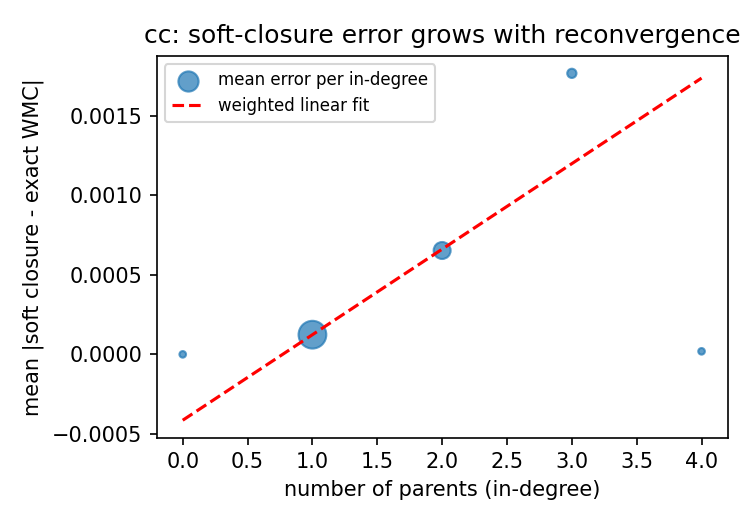
\includegraphics[width=\columnwidth]{fig_cc_error_vs_indegree.png}
\caption{Per-term soft-closure error on GO cc against in-degree. Marker area is term count; dashed line is a count-weighted linear fit.}\label{fig:indegree}
\end{figure}

\paragraph{Modular exact WMC.}
Separator-aware modular WMC gives Table~\ref{tab:modular}. Monolithic $\tw$ is $12/37/269$ for cc/mf/bp; after cutting reconvergence cores of 0\%/5.0\%/9.0\%, we obtain exact marginals for 100\%/95.0\%/91.0\% of terms in 1/6{,}519/7{,}249 modules (max augmented $\tw$ 12/5/12; wall times 3.0\,s/57\,s/379\,s). Every validated module matches brute force to $5.6{\times}10^{-17}$.

\begin{table}[t]\centering
\caption{Separator-aware modular exact WMC on GO and additional ontologies. GO rows are the three standard namespaces (cc/mf/bp = cellular component / molecular function / biological process). ``Core'' is the boundary-aware reconvergence core. ``Exact'' is the fraction of terms solved exactly in augmented modules $M\cup B$.}\label{tab:modular}
\footnotesize
\setlength{\tabcolsep}{2.5pt}
\resizebox{\columnwidth}{!}{%
\begin{tabular}{@{}lrrrrrrr@{}}
\toprule
Ontology & terms & \%mp & $\tw$ & core & mods & $\tw_{\max}$ & exact \\
\midrule
GO cc    & 4041  & 13\% & 12  & 0.0\% & 1     & 12 & 100.0\% \\
GO mf    & 10131 & 20\% & 37  & 5.0\% & 6519  & 5  & 95.0\% \\
GO bp    & 25950 & 53\% & 269 & 9.0\% & 7249  & 12 & 91.0\% \\
UBERON   & \tbd  & \tbd & \tbd & \tbd  & \tbd  & \tbd & \tbd \\
ChEBI    & \tbd  & \tbd & \tbd & \tbd  & \tbd  & \tbd & \tbd \\
\bottomrule
\end{tabular}}
\end{table}

\paragraph{Rank-$r$ separator and NF2.}
On GO residual cores, rank-1 boundary messages discard median $\mathrm{KL}(q^\star\Vert\text{product})=1.49$ nats over the 40 highest-degree cc cores; a representative $10$-term core is exact at tensor-train rank $6$ (Table~\ref{tab:rank}). Core-term marginals under rank-1 err by up to $8.5\times10^{-2}$ (cc) and $3.6\times10^{-1}$ (bp) and become exact to $10^{-15}$ at full separator rank. Adding conjunction definitions (NF2) yields 99\%/97\%/83\% exact on GO cc/mf/bp at 1\%/3\%/17\% cores (Appendix~\ref{app:multi-ontology}).

\subsection{UBERON and ChEBI}\label{sec:other-ont}
Table~\ref{tab:ontology-struct} reports structure statistics for all three ontologies. Greedily cutting the top 5\% highest-degree terms collapses residual treewidth sharply (GO bp: $269\!\to\!12$). Full modular-pipeline results for UBERON and ChEBI are in Table~\ref{tab:modular}.

\begin{table}[t]\centering
\caption{Cross-ontology structure probe (EL\textsuperscript{++} true-path compilation). ``Res.\ $\tw$@5\%'' is residual treewidth after cutting the top 5\% highest-degree terms.}\label{tab:ontology-struct}
\footnotesize
\setlength{\tabcolsep}{2.5pt}
\resizebox{\columnwidth}{!}{%
\begin{tabular}{@{}lrrrrr@{}}
\toprule
Ontology & terms & \%mp & max in-deg & $\tw$ & res.\ $\tw$@5\% \\
\midrule
GO cc  & 4041  & 13\% & 4 & 12  & \tbd \\
GO mf  & 10131 & 20\% & 7 & 37  & \tbd \\
GO bp  & 25950 & 53\% & 9 & 269 & 12 \\
UBERON & \tbd  & \tbd & \tbd & \tbd & \tbd \\
ChEBI  & \tbd  & \tbd & \tbd & \tbd & \tbd \\
\bottomrule
\end{tabular}}
\end{table}

\subsection{Downstream GO Protein-Function Prediction}\label{sec:downstream}
We apply the layer as a drop-in posterior without retraining the base predictor. Base marginals $p_i$ come from \tbd\ (e.g., DeepGOPlus / ESM2+GO). Table~\ref{tab:downstream} reports hierarchy violation rate, F-max, and AUPR on a standard CAFA-style split.

\begin{table}[t]\centering
\caption{Downstream GO protein-function prediction (\tbd\ predictor, \tbd\ split).}\label{tab:downstream}
\footnotesize
\setlength{\tabcolsep}{3pt}
\begin{tabular}{@{}lccc@{}}
\toprule
Method & Violation rate & F-max & AUPR \\
\midrule
Raw $p_i$ & \tbd & \tbd & \tbd \\
Soft closure & \tbd & \tbd & \tbd \\
Modular exact (rank-1) & \tbd & \tbd & \tbd \\
Modular exact (full rank) & \tbd & \tbd & \tbd \\
\bottomrule
\end{tabular}
\end{table}

\subsection{Comparison with NeSy Baselines}
Table~\ref{tab:nesy} fills in the quantitative cells sketched in Table~\ref{tab:inference-routes}: drift vs.\ exact WMC on matched true-path subgraphs with identical priors. DeepProbLog compiles GO cc ($\tw{=}12$) but not mf/bp ($2^{37}$/$2^{269}$). Scallop scales to full GO bp but undercounts at reconvergences when $k$ is small (max drift $0.34$ at $k{=}1$). A-NeSI is evaluated on carry chains only (Appendix~\ref{app:nesy}).

\begin{table}[t]\centering
\caption{NeSy frameworks on matched true-path subgraphs. A-NeSI/NeSyDM need per-ontology training and exact-$\WMC$ samples.}\label{tab:nesy}
\footnotesize
\setlength{\tabcolsep}{1.5pt}
\resizebox{\columnwidth}{!}{%
\begin{tabular}{@{}llccc@{}}
\toprule
Method & Evaluated on & Full ont. & Mean drift & Max drift \\
\midrule
DeepProbLog & GO cc/mf/bp & No & 0 (exact) & 0 (exact) \\
Scallop ($k{=}1$) & GO bp & Yes & \tbd & 0.34 \\
Scallop ($k{=}10$) & GO bp & Yes & \tbd & $<10^{-3}$ \\
A-NeSI / NeSyDM & Carry chain & No & \tbd & \tbd \\
Ours (modular) & GO cc/mf/bp & Yes & \tbd & \tbd \\
Ours (modular) & UBERON & \tbd & \tbd & \tbd \\
Ours (modular) & ChEBI & \tbd & \tbd & \tbd \\
\bottomrule
\end{tabular}}
\end{table}

\subsection{Transfer and Limits}\label{sec:transfer}
We test whether the GO-tuned core-selection heuristic ($\tw_{\max}{=}14$) transfers to UBERON and ChEBI without retuning (Table~\ref{tab:transfer}). Failure modes include inexact rank-1 core terms, NF2-induced treewidth growth, and the SROIQ disjunctive regime (Appendix~\ref{app:nesy}).

\begin{table}[t]\centering
\caption{Transfer of core-selection heuristic (no retuning). ``$\Delta$ exact'' is change vs.\ ontology-tuned core budget.}\label{tab:transfer}
\footnotesize
\setlength{\tabcolsep}{3pt}
\begin{tabular}{@{}lccc@{}}
\toprule
Ontology & GO-tuned exact & Tuned exact & $\Delta$ exact \\
\midrule
UBERON & \tbd & \tbd & \tbd \\
ChEBI  & \tbd & \tbd & \tbd \\
\bottomrule
\end{tabular}
\end{table}

\section{Conclusion}\label{sec:conclusion}
We characterize the soft closure deployed in NeSy systems as loopy belief propagation on hierarchical ontology constraints: exact on tree-like structure and wrong only at reconvergences. Separator-aware modular exact WMC recovers exact marginals on most concepts by isolating a small reconvergence core; a rank-$r$ separator interpolates between the fast closure and exact inference. On Gene Ontology, cutting 0--9\% cores yields 91--100\% modular-exact coverage across the cc, mf, and bp namespaces; the same pipeline extends to UBERON and ChEBI. The layer maps independent predictor scores to structure-aware marginals without retraining. Remaining limits include full SROIQ disjunction, rank-1 error on reconvergent cores, and learned approximators that require per-ontology training.

\section{Ethical Statement}
This work uses publicly available ontologies (GO, UBERON, ChEBI) and poses no human-subjects risk. Improved ontology consistency may affect automated annotation quality. Users should treat $\mu_i$ as a structural correction layer, not a standalone clinical predictor.

\paragraph{Data availability.}
Code, data, Lean developments, and experiment scripts will be released upon publication.

\bibliography{references}

\appendix

\section{Application Note}
The inference layer is a drop-in posterior. Independent neural marginals $p_i$ map to structure-conditioned $\mu_i$ with no retraining, useful for GO-based function predictors \citep{kulmanov2020deepgoplus,lin2023esm2,yu2023clean,kulmanov2018deepgo,kulmanov2022deepgozero} and, more broadly, any hierarchical ontology predictor that outputs per-concept scores.

\section{Multi-ontology experiment details}\label{app:multi-ontology}

\paragraph{Ontology releases and preprocessing.}
GO \citep{geneontology2023}: \texttt{go-basic} release of June 2025 (\texttt{go-basic.obo}); namespaces cc, mf, bp as above. UBERON \citep{mungall2012uberon}: release \tbd, non-obsolete \emph{is-a} backbone after EL\textsuperscript{++} normalization. ChEBI \citep{hastings2016chebi}: release \tbd, same pipeline. All ontologies are compiled with the ELK reasoner normal forms \citep{kazakov2014elk}.

\paragraph{Structure and downstream (GO, UBERON, ChEBI).}
\begin{itemize}
\item[\checkmark] GO cc/mf/bp structure statistics (partial: Table~\ref{tab:ontology-struct}).
\item[\ ] UBERON/ChEBI: terms, \%mp, max in-degree, monolithic $\tw$, residual $\tw$@1/5/9\% cuts.
\item[\ ] Per-ontology soft-closure error vs.\ in-degree plots (GO cc: Fig.~\ref{fig:indegree}; UBERON/ChEBI: \texttt{fig\_uberon\_error\_vs\_indegree.png}, \texttt{fig\_chebi\_error\_vs\_indegree.png}).
\item[\ ] Downstream Table~\ref{tab:downstream}: pick predictor (\tbd), split (\tbd), report violation/F-max/AUPR.
\end{itemize}

\paragraph{Full pipeline and NeSy baselines.}
\begin{itemize}
\item[\checkmark] GO modular exact WMC (Table~\ref{tab:modular}).
\item[\ ] UBERON full modular pipeline: core\%, modules, $\tw_{\max}$, exact\%, wall time.
\item[\ ] ChEBI full modular pipeline (same columns).
\item[\ ] NF2 extension on all five rows (GO cc/mf/bp + UBERON + ChEBI).
\item[\ ] Unified NeSy Table~\ref{tab:nesy}: Scallop mean drift on matched GO bp subgraphs; DeepProbLog compile limits per ontology.
\end{itemize}

\paragraph{Transfer and limits.}
\begin{itemize}
\item[\ ] Table~\ref{tab:transfer}: GO-tuned vs.\ tuned core budget on UBERON/ChEBI.
\item[\ ] Failure case study: list top-$k$ inexact terms under rank-$1$ on GO bp and ChEBI.
\item[\ ] Reproducibility: anonymized repo with one-command reproduce per ontology (\tbd\ URL).
\end{itemize}

\section{Formalisation: implementation and lemma inventory}\label{app:lean}

\paragraph{A kernel-checked development with decidable rational arithmetic.}
The Lean~4 development (\texttt{Wmc.lean}, Lean 4.31) is a single Lean-core file with no
dependence on \texttt{mathlib}. It defines worlds as Boolean lists, the true-path constraint
as a conjunction of edge clauses $(\neg y_c \vee y_\pi)$, the exact weighted model count as a
ratio of summed world weights (\texttt{marginal}), and the soft-OR update (\texttt{softOR}),
and it closes every claim by \texttt{decide}, reduction in the kernel, with no
\texttt{native\_decide} escape hatch and therefore no trust placed in compiled code. To keep
rational arithmetic cheap in the kernel we use a \emph{custom rational encoding}. A rational
is a pair $Q=\mathbb{Z}\times\mathbb{Z}$ of numerator and denominator, with addition,
multiplication and complementation ($1-a$) defined directly on the pair, and equality the
\emph{cross-multiplied} test $a_1 b_2 = b_1 a_2$, decidable on integers without normalizing the
fraction. Hence world enumeration, weighting, summation, and the soft-OR/WMC comparison are all
reducible by \texttt{decide}. \texttt{\#print axioms} reports every theorem depends on
$\{\texttt{propext}\}$ alone, with no \texttt{Classical.choice}, no \texttt{Quot.sound}, no
\texttt{sorry}.

\paragraph{Parametric development and lemma inventory.}
The general Theorem~\ref{thm:star}, over all $k:\mathbb{N}$ and all real priors, is proved in a
separate \texttt{mathlib} development (\texttt{WmcStar.star\_marginal\_eq\_softOR}, Lean 4.31).
It models worlds as \texttt{Bool}\,$\times$\,(\texttt{Fin}\,$k\to$\texttt{Bool}), uses the
product-of-sums interchange \texttt{Finset.prod\_univ\_sum} to evaluate the parent-true mass to
$q_\pi$ and \texttt{Finset.sum\_eq\_single} to collapse the parent-false case to the all-false
world, giving $Z=q_\pi+(1-q_\pi)\prod_i(1-q_i)$ and the soft-OR ratio. Its axiom footprint is
$\{\texttt{propext},\texttt{Classical.choice},\texttt{Quot.sound}\}$ with no \texttt{sorry}. The
concrete Lean-core development additionally checks the instances directly. The single edge
(\texttt{single\_edge\_exact}) and the $k{=}2,3$ stars (\texttt{star2\_exact},
\texttt{star3\_exact}) reduce both sides to the same $Q$ by \texttt{decide}. The reconvergence is the diamond
($d\!\Rightarrow\!b,c$, $b,c\!\Rightarrow\!a$). \texttt{diamond\_exact\_5\_6} proves the exact
reconvergent marginal is $5/6$. \texttt{diamond\_softor\_9\_10} proves the soft-OR update (the
two paths merged independently) is $9/10$. \texttt{diamond\_softor\_ne\_exact} proves they
are unequal, so the soft closure is exact on the tree fragment and provably inexact at the
reconvergence. Unconditional convergence of the monotone closure is the finite-vocabulary
least-fixpoint argument of \S\ref{sec:lean} (the synchronous step is extensive and monotone, so
it stabilizes within the graph depth). We verify the exact/soft values rather than re-prove the
fixpoint in Lean.

\section{Extended neuro-symbolic comparison numbers}\label{app:nesy}

\paragraph{Top-$k$ provenance (Scallop).}
The four-node reconvergent derivation has two proof paths to a shared fact via the upward rule $\texttt{holds}(P)\!:\!-\,\texttt{sub}(C,P),\texttt{holds}(C)$ at edge-probability $\tfrac12$, a construction distinct from the Lean true-path diamond of \S\ref{sec:lean} (different inference semantics, so its exact value $0.9375$ does not conflict with $5/6$ on that diamond). Run in the actual Scallop system (\texttt{scallopy}, built from source, top-$k$-proofs), the exact marginal $P(\texttt{holds}(a))=0.9375$ is returned as $0.50$ at $k{=}1$ (a $47\%$ undercount), $0.875$ at $k{=}3$, and the exact $0.9375$ at $k{=}10$, identical to our exact-semantics reference. On real biological-process neighbourhoods the maximum drift versus the exact provenance reference falls from $0.34$ at $k{=}1$ (over 200 targets, $0.21$ on a $14$-term cone run in \texttt{scallopy}) to below $10^{-3}$ at $k{=}10$. The error therefore grows with proof multiplicity (reconvergence) and shrinks as $k$ admits more proofs, the same reconvergence axis along which our soft closure departs from exact $\WMC$.

\paragraph{The carry-chain: exact independence vs.\ its sampled estimate.}
We instantiate the $N$-digit carry chain as MNIST addition under distant (sum-only) supervision,
training a shared digit CNN with the independence-assumption marginal of the sum and reporting
test sum-accuracy over three seeds. With the \emph{exact} independence product (computed by
convolving the per-position digit distributions) the model degrades only gently as the carry
couples more digits: $0.970/0.942/0.926/0.905$ for $N{=}1$ to $4$, the per-digit error
compounding rather than a collapse. Its bare \emph{Monte-Carlo} estimate, the sampling a naive
learned objective rests on, instead collapses over the same range, $0.129/0.010/0.001/0.000$,
as the probability that a sample satisfies the constraint vanishes and the gradient disappears.
This is the independence-assumption / reasoning-shortcut failure
\citep{vankrieken2024independence,marconato2023reasoningshortcuts} that learned inference engines
are built to escape, and they do. Run in the \emph{actual} A-NeSI system on the same benchmark
($20$ epochs/seed), sum-accuracy is $0.973/0.922/0.875/0.748$ from $N{=}1$ to $4$, a graceful
degradation tracking the exact product, not the collapse of the sampler, because A-NeSI learns the
inference distribution rather than sampling the constraint. The cost is moved, not removed. Neither
A-NeSI nor NeSyDM \citep{vankrieken2025nesydm} can be run on GO (each needs a model trained per
ontology, and A-NeSI needs samples of the exact $\WMC$ we compute), which is exactly what the
training-free exact construction of this paper supplies.

\paragraph{Boundary-rank dial on the GO cc reconvergence core (\S\ref{sec:scaling}).}
The exact constraint-induced boundary joint over a real GO cc reconvergence core ($10$ terms from the June 2025 \texttt{go-basic} release, $53$ models, exact tensor-train rank $6$) is strongly non-product. A rank-$r$ separator message, a tensor train over the separator atoms with the per-module circuits fixed, dials the residual to zero. The rank-$1$ row is exactly the independent soft closure (Table~\ref{tab:rank}).

\begin{table}[t]\centering
\caption{A rank-$r$ separator message dials the residual-core error to zero (real GO cc reconvergence core, $10$ terms, per-module circuits fixed). $q^\star$ is the exact constraint-induced boundary joint. ``Gap closed'' is the fraction of the rank-$1$ total variation removed.}\label{tab:rank}
\footnotesize
\setlength{\tabcolsep}{3pt}
\begin{tabular}{@{}lccc@{}}
\toprule
Boundary head & KL & TV & Gap closed\\
\midrule
rank-$1$ (indep.) & $1.95$ & $0.68$ & -- \\
rank-$2$ & $1.46$ & $0.36$ & $46\%$\\
rank-$4$ & $0.26$ & $0.12$ & $82\%$\\
rank-$6$ (full) & $0.00$ & $0.00$ & exact\\
\bottomrule
\end{tabular}
\end{table}

\paragraph{The dial is systematic across cores.}
Over the $40$ highest-degree multi-parent cc cores (upper cones of up to $13$ terms), the
constraint-induced boundary joint is non-product in every case. The IA gap
$\mathrm{KL}(q^\star\Vert\text{product})$ is $1.49$ nats in the median (range $0.54$--$3.75$).
The exact rank of the joint is $5$ in the median (range $3$--$10$), always far below the $2^{w}$
dense size. The single core of Table~\ref{tab:rank} is representative, not cherry-picked.

\paragraph{The disjunctive (SROIQ) regime: a multimodal joint.}
The monotone true-path theory gives a unimodal, merely correlated boundary joint. Disjunction is the
qualitative break. On a controlled fragment over $w{=}6$ boundary atoms, two entities, each typed by
an exactly-one-of-three axiom (covering $+$ pairwise disjointness), coupled by cross-entity
disjointness, the exact joint is \emph{multimodal} ($6$ modes), and the IA cannot represent it.
The best product discards $2.03$ nats (total variation $0.87$, $11\%$ error on a composed query). The
rank-$r$ dial is exact only at full rank $3$ of the joint (Table~\ref{tab:disj}). This is the
regime that the disjoint-cube result of van Krieken rules out for the IA, and the one a SROIQ extension targets.

\begin{table}[t]\centering
\caption{Cost-II in the disjunctive (SROIQ) regime: covering $+$ disjointness over $w{=}6$ atoms give a $6$-mode joint the IA cannot represent. A rank-$r$ separator message is exact at full rank $3$ of the joint. ``WMC rel.\ err.'' is the relative error on a composed query $P(a_1\vee b_2)$.}\label{tab:disj}
\footnotesize
\setlength{\tabcolsep}{3pt}
\begin{tabular}{@{}lccc@{}}
\toprule
Boundary model & KL & TV & WMC rel.\ err.\\
\midrule
IA (best product) & $2.03$ & $0.87$ & $1.1{\times}10^{-1}$\\
rank-$2$ & $0.38$ & $0.28$ & $4.1{\times}10^{-2}$\\
rank-$3$ (full) & $0.00$ & $0.00$ & $0$\\
\bottomrule
\end{tabular}
\end{table}

\end{document}
